% ============================================================================
%  Final Project, Iteration 3
%  Movie Recommender with Matrix Factorization: ALS vs. Truncated SVD
%
%  Same style as the Iteration 2 report (main.tex); kept as a separate file
%  so that both reports stay intact.
%
%  Figures: upload these PNGs from the repository's figures/ folder into a
%  figures/ folder in this Overleaf project:
%    als_objective_simulation.png  als_error_vs_size.png  als_stress_test.png
%    als_test_rmse_real.png        als_objective_real.png
%    assumptions_simulation.png    assumptions_real.png
%
%  \tbd{...} (red) and the red boxes mark what the team still has to fill in.
%  Every number in this file was produced by src/small_example.py,
%  src/check_simulation.py or src/run_real.py.
% ============================================================================
\documentclass[11pt]{article}
\usepackage[letterpaper,margin=1in]{geometry}
\usepackage{amsmath,amssymb,amsthm}
\usepackage{booktabs,array,enumitem}
\usepackage{graphicx}
\usepackage{float}
\usepackage{xcolor}
\usepackage[hidelinks]{hyperref}

\newtheorem{proposition}{Proposition}
\theoremstyle{definition}
\newtheorem{remark}[proposition]{Remark}
\setcounter{proposition}{8}   % Propositions 1--8 are in the Iteration 2 report

\newcommand{\R}{\mathbb{R}}
\newcommand{\T}{^{\top}}
\newcommand{\Iu}{\mathcal{I}_u}
\newcommand{\Ui}{\mathcal{U}_i}
\newcommand{\code}[1]{\texttt{#1}}
\newcommand{\tbd}[1]{\textcolor{red}{[#1]}}
\newcommand{\owner}[2]{\par\smallskip\noindent\hfill
  {\footnotesize\itshape Owner: #1\enspace$\bullet$\enspace Checked by: #2}\par\medskip}
\newcommand{\placeholder}[2]{\par\medskip\noindent
  \fbox{\parbox{\dimexpr\linewidth-2\fboxsep-2\fboxrule\relax}{\color{red}
  \textbf{To be added by #1.} #2}}\par\medskip}

\title{DS5020 Final Project -- Iteration 3\\[4pt]
  \large Movie Recommender with Matrix Factorization: ALS vs.\ Truncated SVD}
\author{Muhammad Saad Malik \and Jagadeesh Aravind Kalyan Shetti \and Emmanuel Adjei Danso}
\date{Fall 2026}

\begin{document}
\maketitle

In Iteration~2 we derived our methods and checked every result on simulated data. In this
iteration we turn the mathematics into code written from scratch and verify it at three levels.
A $3\times 3$ example worked step by step in exact fractions tests that we understand every step;
a simulation in which the true answer is known tests that the method is correct; and MovieLens
100K tests that it works in practice, with every from-scratch result compared against a library.
Section~\ref{sec:changes} lists what changed since Iteration~2 and why. Section~\ref{sec:impl}
maps each step of the ALS algorithm (Method~2) to the function that computes it.
Sections~\ref{sec:example}--\ref{sec:real} contain the worked example, the simulation test and
the real-data results, Section~\ref{sec:assumptions} checks the assumptions of Iteration~2 on
both data sets, Section~\ref{sec:questions} answers the Iteration~3 math questions, and
Section~\ref{sec:verification} collects every comparison in one verification table.
Propositions~1--8 and Theorem~4 refer to the Iteration~2 report, and the numbering continues
from there.

% ============================================================================
\section{Changes since Iteration 2}
\label{sec:changes}

The handout asks us to keep the dataset, simulation model, parameter values and random seed of
Iteration~2, and to say why if any of them changes. The simulated data are identical: the new
function \code{simulate\_ratings} makes the same random draws in the same order as Iteration~2,
and gives the same $|\Omega| = 2{,}281$ observed entries. Table~\ref{tab:changes} lists what did
change.

\begin{table}[htbp]
\centering
\small
\begin{tabular}{@{}>{\raggedright}p{2.3cm}>{\raggedright}p{3.5cm}>{\raggedright}p{4.2cm}>{\raggedright\arraybackslash}p{5.0cm}@{}}
\toprule
What & Iteration 2 & Iteration 3 & Why \\
\midrule
Solving the $k\times k$ systems & \code{numpy.linalg.solve} & Our own Gaussian elimination
  with partial pivoting (Section~\ref{sec:gauss}) & The core method must use only NumPy arrays and
  matrix products; libraries are allowed only as a check. \\
\addlinespace
Starting factors (Step~2) & Standard normal entries, drawn from the same generator as the data
  & Entries from $\mathcal N(0, 0.1^2)$, drawn from \code{default\_rng(0)} inside the ALS function
  & Matches ``small random entries'' in Step~2, and the start no longer depends on how many random
  numbers the data used. \\
\addlinespace
Centring (Step~1) in the simulation & Not applied & Applied ($\mu = 0.0202$) & The same
  functions now run every data set, exactly as Method~2 is written. \\
\addlinespace
Train/test split & Our seeded 80/20 split of \code{u.data} & The provided split
  \code{u1.base} / \code{u1.test} & Required by the handout, so that results are comparable across
  teams. \\
\addlinespace
Ranks and $\lambda$ & $k \in \{1,2,5,10,20,50\}$ & $k \in \{2,5,10,20\}$ and
  $\lambda \in \{0.1, 1, 10\}$ & The grid set by the handout. \\
\addlinespace
Stopping rule (Step~6) & ``A tolerance or a fixed number of sweeps'' & At most 50 sweeps, or stop
  when one sweep lowers $J$ by less than $10^{-5}J$ & Made concrete for the code. \\
\addlinespace
Simulation code & One script, \code{simulation.py} & The data model as a function in
  \code{simulate.py}; the checks in \code{check\_simulation.py} & Required by the handout; lets the
  same model run at any size or observed fraction. \code{simulation.py} is kept as the record of
  Iteration~2. \\
\bottomrule
\end{tabular}
\caption{What changed since Iteration~2, and why.}
\label{tab:changes}
\end{table}

\paragraph{Effect on the simulation.} The data are unchanged, so only the path that ALS takes
changes: $J$ now starts at 7{,}112.18 instead of 14{,}549.15 and ends at 547.09 instead of 546.68,
and the error on the hidden entries is 0.150 instead of 0.147. Both are far below the pass
threshold of 0.3.

\paragraph{Effect on the real data.} The provided split is harsher than ours. The user with the
fewest training ratings has 4 instead of 13, 32 movies have no training ratings at all, and 32
test ratings fall on those movies (40 in Iteration~2). Assumption~4 and Proposition~2 therefore
matter even more than before (Section~\ref{sec:a4}).

% ============================================================================
\section{The Implementation}
\label{sec:impl}

The core method is in \code{src/methods.py}. It uses only NumPy arrays, matrix products and our
own Gaussian elimination; \code{numpy.linalg} appears only in the scripts that check the answers.
Each step of Method~2 (Iteration~2, Section~6.2) is one function, with the equation it computes
written as a comment above it in the symbols of our notation table. Table~\ref{tab:steps} gives
the correspondence.

\begin{table}[htbp]
\centering
\small
\begin{tabular}{@{}c>{\raggedright}p{8.6cm}>{\raggedright\arraybackslash}p{4.6cm}@{}}
\toprule
Step & What it computes & Function \\
\midrule
1 & $\mu = \frac{1}{|\Omega_{\mathrm{tr}}|}\sum_{(u,i)\in\Omega_{\mathrm{tr}}} r_{ui}$;
    the factors are fitted to $r_{ui} - \mu$ & \code{my\_centre} \\
2 & $U^{(0)} \in \R^{m\times k}$, $V^{(0)} \in \R^{n\times k}$ with entries from
    $\mathcal N(0, 0.1^2)$, seed 0 & \code{my\_init\_factors} \\
3 & For every user: $G_u u_u = h_u$ with $G_u = V_u\T V_u + \lambda I_k$ and
    $h_u = V_u\T r_u$ (Proposition~1) & \code{my\_update\_U}, using
    \code{my\_normal\_equations} and \code{my\_gauss\_solve} \\
4 & For every movie: $(U_i\T U_i + \lambda I_k)\, v_i = U_i\T r_{(i)}$ & \code{my\_update\_V} \\
5 & $J(U,V)$ after every half-step; an increase stops the run with an error (Theorem~4)
  & \code{my\_objective}, check in \code{my\_als} \\
6 & Repeat Steps 3--5: at most 50 sweeps, or until one sweep lowers $J$ by less than $10^{-5}J$
  & \code{my\_als} \\
7 & $\hat r_{ui} = \mu + u_u\T v_i$, clipped to $[1,5]$ & \code{my\_predict} \\
-- & $\mathrm{RMSE} = \bigl(\frac1N \sum (\hat r_{ui} - r_{ui})^2\bigr)^{1/2}$ over a set of
    pairs & \code{my\_rmse} \\
\bottomrule
\end{tabular}
\caption{Each step of Method~2 and the function in \code{src/methods.py} that computes it.}
\label{tab:steps}
\end{table}

Step~4 needs no code of its own. Exchanging users and movies turns $R \approx UV\T$ into
$R\T \approx VU\T$ (Proposition~1, Step~5), so \code{my\_update\_V} calls \code{my\_update\_U} on
the transposed data. A user or movie with no ratings gets $G = \lambda I_k$ and $h = 0$, hence the
zero vector, and is predicted at $\mu$.

Every function also accepts NumPy arrays of Python \code{Fraction} objects. The worked example of
Section~\ref{sec:example} therefore runs on exactly the same code as the simulation and the real
data, but in exact rational arithmetic.

\subsection{\texorpdfstring{Solving the $k\times k$ systems}{Solving the k x k systems}}
\label{sec:gauss}

Each sweep solves $m + n$ systems of size $k\times k$: 2{,}625 of them on MovieLens.
\code{my\_gauss\_solve} solves $Gx = h$ by Gaussian elimination with partial pivoting:
\begin{enumerate}[leftmargin=*]
  \item Form the augmented matrix $A = [\,G \mid h\,] \in \R^{k\times(k+1)}$.
  \item \emph{Forward elimination.} For $c = 1, \dots, k$: swap row $c$ with the row
        $p = \arg\max_{r \ge c} |a_{rc}|$, then for every $r > c$ replace row $r$ by
        row $r - (a_{rc}/a_{cc})$ row $c$. All rows below the pivot are updated at once, as one
        outer product.
  \item \emph{Back substitution.} For $r = k, \dots, 1$:
        $x_r = \bigl(a_{r,k+1} - \sum_{j > r} a_{rj}\, x_j\bigr) / a_{rr}$.
\end{enumerate}
This costs about $\tfrac23 k^3$ multiply--adds, the count used in Iteration~2. A full ALS run of
50 sweeps on MovieLens took at most 13 seconds on a laptop, at $k = 20$.

\begin{proposition}[Elimination never meets a zero pivot]
\label{prop:pivot}
For $\lambda > 0$, Gaussian elimination with partial pivoting applied to
$G_u = V_u\T V_u + \lambda I_k$ finds a nonzero pivot in every column, so \code{my\_gauss\_solve}
always returns the unique solution of $G_u u_u = h_u$.
\end{proposition}

\begin{proof}
\textbf{Step 1: row operations keep the matrix invertible.} A row swap, and replacing row $r$ by
row $r$ minus a multiple of row $c$, are each multiplication on the left by an invertible
elementary matrix. After any number of them the matrix is $EG_u$ with $E$ invertible. By
Proposition~2, $G_u$ is invertible, and so is $EG_u$.

\textbf{Step 2: a zero column would make it singular.} Suppose that at column $c$ every entry on or
below the diagonal were zero. Each of the first $c - 1$ columns already has zeros below its
diagonal entry, so all of the first $c$ columns would have nonzero entries only in rows
$1, \dots, c-1$. That is $c$ vectors in a space of dimension $c - 1$, so they would be linearly
dependent and $EG_u$ would be singular, contradicting Step~1. Hence the largest $|a_{rc}|$ with
$r \ge c$ is nonzero.

\textbf{Step 3: the answer is the unique solution.} Back substitution divides only by these
nonzero pivots. Every row operation is invertible, so the triangular system has the same
solutions as $G_u u_u = h_u$, and since $G_u$ is invertible that solution is unique.
\end{proof}

\begin{remark}[How large the rounding error should be]
\label{rem:rounding}
Every eigenvalue of $G_u$ is at least $\lambda$ (Proposition~2), so its condition number
$\operatorname{cond}(G_u) = \gamma_{\max}/\gamma_{\min}$ is at most $\gamma_{\max}/\lambda$.
Gaussian elimination with partial pivoting is backward stable in practice: it returns the exact
solution of a system very close to the one given. Two such solvers can therefore disagree by about
$\operatorname{cond}(G_u)\,\varepsilon$ in relative terms, where
$\varepsilon \approx 2.2\times 10^{-16}$ is the machine epsilon. This is the scale against which
we judge every comparison with \code{numpy.linalg.solve}.
\end{remark}

\subsection{The files}

\begin{table}[htbp]
\centering
\small
\begin{tabular}{@{}l>{\raggedright\arraybackslash}p{10.8cm}@{}}
\toprule
File in \code{src/} & Role \\
\midrule
\code{methods.py} & The method: one function per step of Method~2 (Table~\ref{tab:steps}) \\
\code{simulate.py} & \code{simulate\_ratings}: the Iteration~2 data model as a function of the
  size, the observed fraction and the seed \\
\code{small\_example.py} & The worked example of Section~\ref{sec:example}, every step printed \\
\code{check\_simulation.py} & The simulation test of Section~\ref{sec:sim} \\
\code{run\_real.py} & The real-data results of Section~\ref{sec:real} \\
\code{assumptions.py} & The assumption checks of Section~\ref{sec:assumptions}, shared by the two
  scripts above \\
\bottomrule
\end{tabular}
\caption{Code for this iteration. The README explains how to run each script.}
\label{tab:files}
\end{table}

\owner{Muhammad Saad Malik}{\tbd{checker}}

% ============================================================================
\section{Small Worked Example}
\label{sec:example}

We take three users, three movies and seven known ratings:
\[
R = \begin{pmatrix} 5 & 4 & ? \\ 4 & ? & 2 \\ 1 & 2 & 1 \end{pmatrix},
\qquad k = 1, \qquad \lambda = 1,
\]
with users as rows and movies as columns. Step~2 normally draws small random entries; here we start
from $v^{(0)} = (1, 1, 1)\T$ so that every number stays a short fraction. Step~1 (centring) is
skipped for the same reason: it would subtract $\mu = 19/7$ from every rating and changes nothing
else in the method. With $k = 1$ every $G_u$ is a $1\times 1$ matrix, so Step~3 becomes the scalar
formula
\[
u_u \;=\; \frac{h_u}{G_u} \;=\; \frac{\sum_{i\in\Iu} v_i\, r_{ui}}{\sum_{i\in\Iu} v_i^2 + \lambda},
\]
which is Proposition~1 with $k = 1$. The numerator collects each rated movie's factor times the
rating it received; the denominator collects the squared factors, plus $\lambda$. Every number
below is printed by \code{src/small\_example.py}.

\paragraph{Step 3: update every user, with $V = v^{(0)}$ fixed.} Table~\ref{tab:ex-users} applies
the formula above to each user in turn.

\begin{table}[H]
\centering
\begin{tabular}{@{}cccccccc@{}}
\toprule
User $u$ & $\Iu$ & $V_u\T$ & $r_u\T$ & $G_u = V_u\T V_u + \lambda$ & $h_u = V_u\T r_u$ & $u_u$ \\
\midrule
1 & $\{1,2\}$   & $(1,1)$   & $(5,4)$   & $1+1+1 = 3$   & $5+4 = 9$     & $3$ \\
2 & $\{1,3\}$   & $(1,1)$   & $(4,2)$   & $1+1+1 = 3$   & $4+2 = 6$     & $2$ \\
3 & $\{1,2,3\}$ & $(1,1,1)$ & $(1,2,1)$ & $1+1+1+1 = 4$ & $1+2+1 = 4$   & $1$ \\
\bottomrule
\end{tabular}
\caption{Step~3 of the worked example.}
\label{tab:ex-users}
\end{table}

So $U^{(1)} = (3, 2, 1)\T$. User~1 rates generously and user~3 harshly, and the single factor
already records this.

\paragraph{Step 5: the objective after Step 3.} Every prediction is $u_u \cdot 1 = u_u$, so
\begin{align*}
\textstyle\sum_{\Omega}\bigl(r_{ui} - u_u v_i\bigr)^2 &= 2^2 + 1^2 + 2^2 + 0^2 + 0^2 + 1^2 + 0^2 = 10,\\
\lambda\bigl(\|U\|_F^2 + \|V\|_F^2\bigr) &= (9 + 4 + 1) + (1 + 1 + 1) = 17,
\end{align*}
and $J\bigl(U^{(1)}, V^{(0)}\bigr) = 27$.

\paragraph{Step 4: update every movie, with $U = U^{(1)}$ fixed.} The same formula with the roles
of users and movies exchanged, using the new $U^{(1)}$ (Table~\ref{tab:ex-movies}).

\begin{table}[H]
\centering
\begin{tabular}{@{}ccccccc@{}}
\toprule
Movie $i$ & $\Ui$ & $U_i\T$ & $r_{(i)}\T$ & $U_i\T U_i + \lambda$ & $U_i\T r_{(i)}$ & $v_i$ \\
\midrule
1 & $\{1,2,3\}$ & $(3,2,1)$ & $(5,4,1)$ & $9+4+1+1 = 15$ & $15+8+1 = 24$ & $8/5$ \\
2 & $\{1,3\}$   & $(3,1)$   & $(4,2)$   & $9+1+1 = 11$   & $12+2 = 14$   & $14/11$ \\
3 & $\{2,3\}$   & $(2,1)$   & $(2,1)$   & $4+1+1 = 6$    & $4+1 = 5$     & $5/6$ \\
\bottomrule
\end{tabular}
\caption{Step~4 of the worked example.}
\label{tab:ex-movies}
\end{table}

So $V^{(1)} = (8/5,\ 14/11,\ 5/6)\T \approx (1.600,\ 1.273,\ 0.833)\T$. Movie~1 received the best
ratings and movie~3 the worst, and their factors are ordered the same way.

\paragraph{Step 5: the objective after Step 4.} The residuals $r_{ui} - u_u v_i$ on the seven known
ratings are
\[
\underbrace{\tfrac15,\ \tfrac{2}{11}}_{\text{user 1}},\qquad
\underbrace{\tfrac45,\ \tfrac13}_{\text{user 2}},\qquad
\underbrace{-\tfrac35,\ \tfrac{8}{11},\ \tfrac16}_{\text{user 3}},
\]
so the squared error is $\tfrac{26}{25} + \tfrac{68}{121} + \tfrac{5}{36}
= \tfrac{189581}{108900} \approx 1.7409$. The penalty is
$14 + \tfrac{64}{25} + \tfrac{196}{121} + \tfrac{25}{36} = \tfrac{2055409}{108900} \approx 18.8743$,
and
\[
J\bigl(U^{(1)}, V^{(1)}\bigr) = \frac{6803}{330} \approx 20.6152.
\]
The two parts moved in opposite directions: the squared error fell from 10 to 1.74 while the
penalty rose from 17 to 18.87. Theorem~4 is about their sum, which fell from 27 to 20.62.

\paragraph{Step 7: predict the missing ratings.} After one iteration,
\[
\hat R = U^{(1)} V^{(1)\top} =
\begin{pmatrix} 24/5 & 42/11 & \mathbf{5/2} \\ 16/5 & \mathbf{28/11} & 5/3 \\ 8/5 & 14/11 & 5/6 \end{pmatrix},
\]
where the bold entries were missing: $\hat r_{13} = 3 \cdot \tfrac56 = 2.5$ and
$\hat r_{22} = 2 \cdot \tfrac{14}{11} \approx 2.55$. User~1 is generous, but movie~3 was rated low
by everyone who saw it, so the prediction is only 2.5.

\paragraph{Checking the result a second way.}
\begin{enumerate}[label=(\alph*), leftmargin=*]
  \item \emph{Substitution.} For all three users and all three movies, $Gx - h = 0$ exactly in
        rational arithmetic; for example $3\cdot 3 - 9 = 0$ for user~1 and
        $15 \cdot \tfrac85 - 24 = 0$ for movie~1. Since $\nabla f_u(u_u) = 2(G_u u_u - h_u)$
        (Proposition~1, Step~3), every new value is a stationary point, and by Proposition~2 the
        unique minimizer.
  \item \emph{Monotonicity.} $J$ fell from 27 to $6803/330$, as Theorem~4 requires.
  \item \emph{More iterations.} Running on in floating point with the same functions, $J$ after
        iterations 1--10 is 20.6152, 18.5226, 17.9993, 17.8536, 17.8122, 17.8004, 17.7971,
        17.7961, 17.7958, 17.7958: it never increases, and settles at 17.796.
\end{enumerate}

\owner{Muhammad Saad Malik}{\tbd{checker}}

% ============================================================================
\section{Simulation Test}
\label{sec:sim}

\code{simulate\_ratings} generates the model of Iteration~2, Section~7.2: $R_{\mathrm{true}} = AB$
with $A \in \R^{100\times 3}$ and $B \in \R^{3\times 80}$ standard normal, noise
$\varepsilon_{ui} \sim \mathcal N(0, 0.1^2)$, and each entry observed with probability 0.3. This
gives $|\Omega| = 2{,}281$ of 8{,}000 entries (28.5\%), with at least 10 ratings for every user and
18 for every movie. We run Method~2, Steps 1--7, with $k = 3$, $\lambda = 1$ and 50 sweeps
($\mu = 0.0202$). The hidden entries of $R_{\mathrm{true}}$ are the truth. Every number in this
section is printed by \code{src/check\_simulation.py}.

\subsection{The objective never increases}

$J$ fell from 7{,}112.18 to 547.09 and did not increase at any of the 100 half-steps; the largest
change between half-steps was $-6.97\times 10^{-7}$ (Figure~\ref{fig:sim-objective}). This is
Theorem~4.

\begin{figure}[htbp]
  \centering
  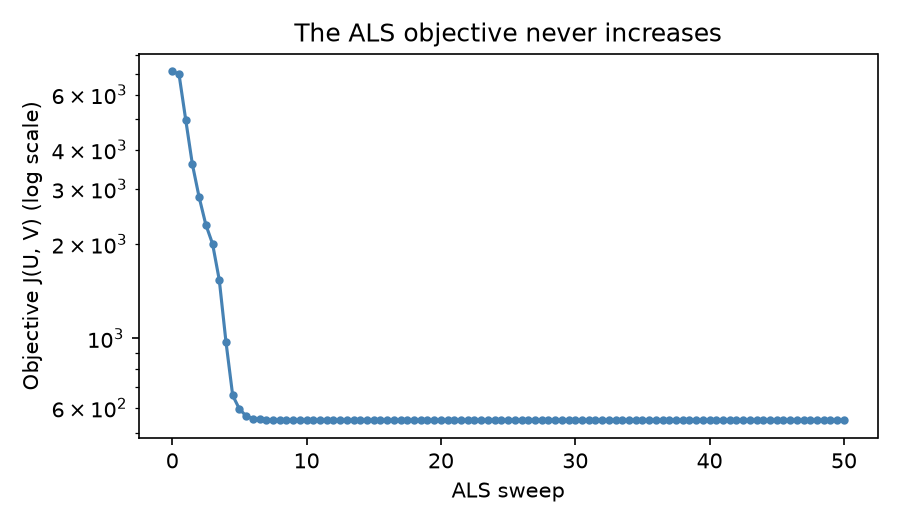
\includegraphics[width=0.62\textwidth]{figures/als_objective_simulation.png}
  \caption{The ALS objective after every half-step of the simulation.}
  \label{fig:sim-objective}
\end{figure}

\subsection{Comparison with the truth}

On the 5{,}719 hidden entries, the RMSE of the predictions against $R_{\mathrm{true}}$ is
\textbf{0.150}, below the pass threshold of 0.3. On the known entries the RMSE against the observed
$R$ is 0.121, slightly above the noise level of 0.1. As in Iteration~2 (0.120), this gap is the
regularization at work: $\lambda$ pulls every factor towards zero.

\subsection{Comparison with the library}

For every one of the 100 user systems and 80 movie systems of the final model we rebuilt $G$ and
$h$ and solved $Gx = h$ both with \code{my\_gauss\_solve} and with \code{numpy.linalg.solve}. For
user~1 the two answers were identical. Over all 180 systems the largest difference was
$8.9\times 10^{-16}$, far below the pass threshold of $10^{-10}$ and of the size
Remark~\ref{rem:rounding} predicts: both solvers compute the same formula and differ only in
rounding.

\subsection{The mean-filled truncated SVD}

Filling the missing entries with $\mu$ and keeping the top three singular triples gives an RMSE of
1.394 on the hidden entries, 9.3 times the error of ALS. This is Q5 of Iteration~2 in numbers: the
SVD fits the 5{,}719 filled-in values as if they were data. This reference value was computed with
\code{numpy.linalg.svd}.

\placeholder{Jagadeesh}{Method~3 from scratch (truncated SVD by power iteration) on the same data:
its $\sigma_1, \dots, \sigma_k$ and singular vectors compared with \code{numpy.linalg.svd} after sign
alignment, its RMSE on the hidden entries, and the swap of the library call in
\code{check\_simulation.py} for the from-scratch function.}

\subsection{Error against sample size}

We kept the model, the observed fraction (30\%) and the seed, and doubled both dimensions of the
matrix three times (Table~\ref{tab:sizes}, Figure~\ref{fig:sizes}). The error on the hidden entries
fell from 0.414 to 0.031, and the slope of $\log(\mathrm{RMSE})$ against $\log|\Omega|$ is $-0.62$.
Larger matrices give every user and movie more ratings, so each system $G_u u_u = h_u$ is fitted
to more data. A slope steeper than the $-\tfrac12$ of pure sampling error is consistent with a
second effect: with $\lambda$ fixed, the shrinkage it causes also fades as each row gets more
ratings.

\begin{table}[htbp]
\centering
\begin{tabular}{@{}rrr@{}}
\toprule
$m \times n$ & $|\Omega|$ & RMSE on hidden entries \\
\midrule
$50 \times 40$   & 592    & 0.4136 \\
$100 \times 80$  & 2{,}281  & 0.1499 \\
$200 \times 160$ & 9{,}601  & 0.0579 \\
$400 \times 320$ & 38{,}283 & 0.0313 \\
\bottomrule
\end{tabular}
\caption{Error against the truth as the matrix grows, 30\% observed, $k = 3$, $\lambda = 1$.}
\label{tab:sizes}
\end{table}

\begin{figure}[htbp]
  \centering
  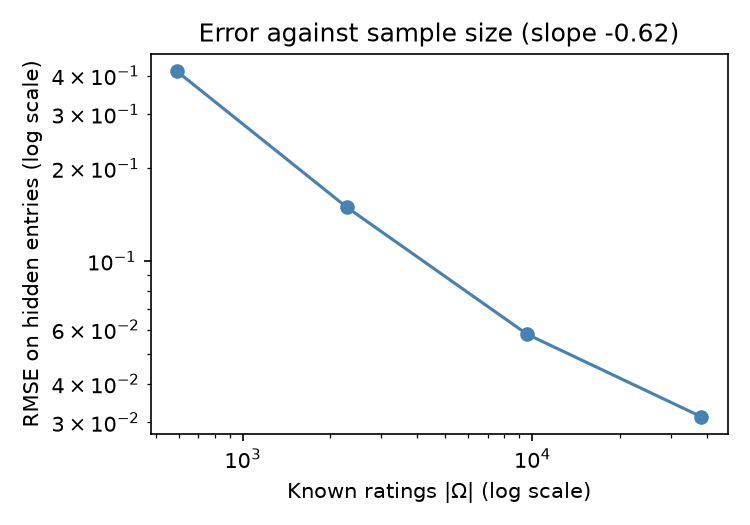
\includegraphics[width=0.52\textwidth]{figures/als_error_vs_size.png}
  \caption{The data of Table~\ref{tab:sizes} on log--log axes; the fitted slope is $-0.62$.}
  \label{fig:sizes}
\end{figure}

\subsection{Stress test: too few known ratings}

We lowered the observed fraction from 30\% to 5\% (Table~\ref{tab:stress},
Figure~\ref{fig:stress}). As a yardstick, ``mean only'' predicts $\mu$ everywhere.

\begin{table}[htbp]
\centering
\begin{tabular}{@{}rrrrrc@{}}
\toprule
Observed & $|\Omega|$ & Fewest ratings for a user & ALS & Mean only & Recovers? \\
\midrule
30\% & 2{,}281 & 10 & 0.150 & 1.764 & yes \\
20\% & 1{,}530 & 6  & 0.280 & 1.762 & yes \\
15\% & 1{,}151 & 4  & 0.419 & 1.760 & no \\
10\% & 815     & 1  & 1.275 & 1.763 & no \\
7\%  & 598     & 1  & 2.001 & 1.765 & no \\
5\%  & 417     & 0  & 1.916 & 1.766 & no \\
\bottomrule
\end{tabular}
\caption{RMSE on the hidden entries as the observed fraction falls ($k = 3$, $\lambda = 1$).
``Recovers'' means an RMSE below 0.3.}
\label{tab:stress}
\end{table}

ALS stops recovering the matrix between 20\% and 15\% observed, and at 7\% and 5\% it does worse
than predicting $\mu$ everywhere. A count of unknowns explains why. The $m\times n$ matrices of
rank $k$ form a set of dimension $k(m + n - k)$: each user and each movie brings $k$ numbers, less
the $k^2$ that the choice $UV\T = (UQ)(VQ^{-\top})\T$ leaves free. Here that is
$3(100 + 80 - 3) = 531$. With 815 ratings there are barely more equations than unknowns, and
with 417 there are fewer, so the data cannot determine the matrix. The same count holds row by
row: a user with one rating cannot pin down three factors. Proposition~2 still guarantees that every
system has a unique solution, but $\lambda$ cannot supply information that the data do not
contain.

\begin{figure}[htbp]
  \centering
  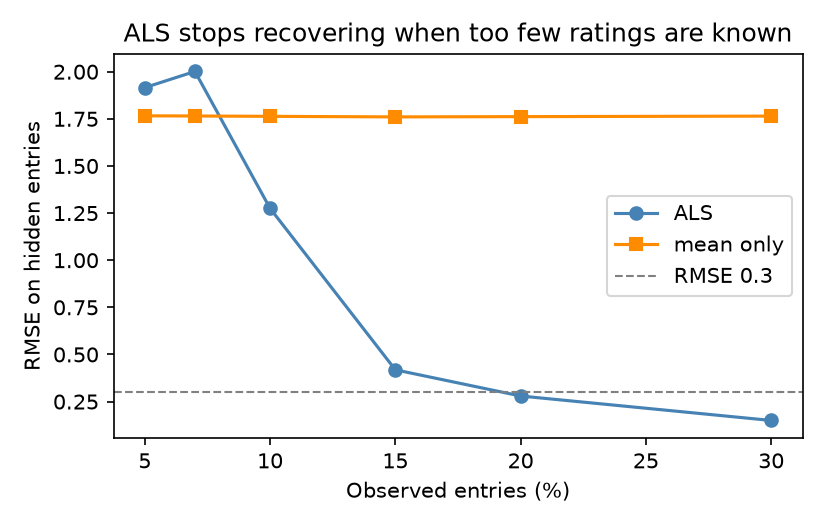
\includegraphics[width=0.56\textwidth]{figures/als_stress_test.png}
  \caption{The data of Table~\ref{tab:stress}. The dashed line is the pass threshold of 0.3.}
  \label{fig:stress}
\end{figure}

\owner{Muhammad Saad Malik}{\tbd{checker}}

% ============================================================================
\section{Real Data: MovieLens 100K}
\label{sec:real}

Every number in this section is printed by \code{src/run\_real.py}.

\subsection{Data and cleaning record}

\begin{itemize}[leftmargin=*]
  \item \textbf{Files.} \code{u1.base} (80{,}000 training ratings) and \code{u1.test} (20{,}000 test
        ratings), on a $943 \times 1682$ matrix. \code{u.data} is used only for the data
        description of Iteration~2.
  \item \textbf{Checks.} Missing values: 0 in each file. Duplicate (user, movie) pairs: 0 in
        each file. Ratings outside 1--5: 0. Pairs in both files: 0.
  \item \textbf{Rows removed:} none.
  \item \textbf{Transformations.} User and movie ids are shifted down by one to become row and
        column indices. Ratings are centred by $\mu = 3.5284$ (Step~1), and predictions are
        clipped to $[1, 5]$ (Step~7). Nothing else is changed.
  \item \textbf{Coverage.} All 943 users and 1{,}650 of the 1{,}682 movies have training ratings.
        No test rating belongs to a user without training ratings; 32 belong to movies without
        any, and are predicted at $\mu$. The fewest training ratings are 4 for a user and 0 for a
        movie; 109 users and 814 movies have fewer than 20.
\end{itemize}

\subsection{Baselines}

Predicting the global mean $\mu$ everywhere gives a test RMSE of 1.1537. Predicting each movie's
mean training rating (or $\mu$ for a movie without training ratings) gives 1.0334. A factorization
that cannot beat 1.0334 has learned nothing about taste.

\placeholder{Emmanuel}{The bias baseline of Method~1, $\hat r_{ui} = \mu + b_u + c_i$, on the same
split, and its test RMSE.}

\subsection{\texorpdfstring{ALS for every $k$ and $\lambda$}{ALS for every k and lambda}}

\begin{table}[htbp]
\centering
\begin{tabular}{@{}rrrrr@{}}
\toprule
$k$ & $\lambda$ & Sweeps & Training RMSE & Test RMSE \\
\midrule
2  & 0.1 & 50 & 0.8737 & 0.9721 \\
5  & 0.1 & 50 & 0.7669 & 0.9947 \\
10 & 0.1 & 50 & 0.6471 & 1.1471 \\
20 & 0.1 & 50 & 0.4664 & 1.2940 \\
\addlinespace
2  & 1   & 23 & 0.8768 & 0.9631 \\
5  & 1   & 50 & 0.7737 & 0.9638 \\
10 & 1   & 50 & 0.6625 & 1.0449 \\
20 & 1   & 50 & 0.4923 & 1.1457 \\
\addlinespace
2  & 10  & 15 & 0.9148 & 0.9837 \\
5  & 10  & 41 & 0.8478 & \textbf{0.9598} \\
10 & 10  & 43 & 0.7905 & 0.9651 \\
20 & 10  & 50 & 0.7165 & 0.9726 \\
\bottomrule
\end{tabular}
\caption{ALS on MovieLens (Method~2, Steps~1--7). ``Sweeps'' is where Step~6 stopped; 50 means the
run reached the sweep limit before the tolerance.}
\label{tab:grid}
\end{table}

\begin{figure}[htbp]
  \centering
  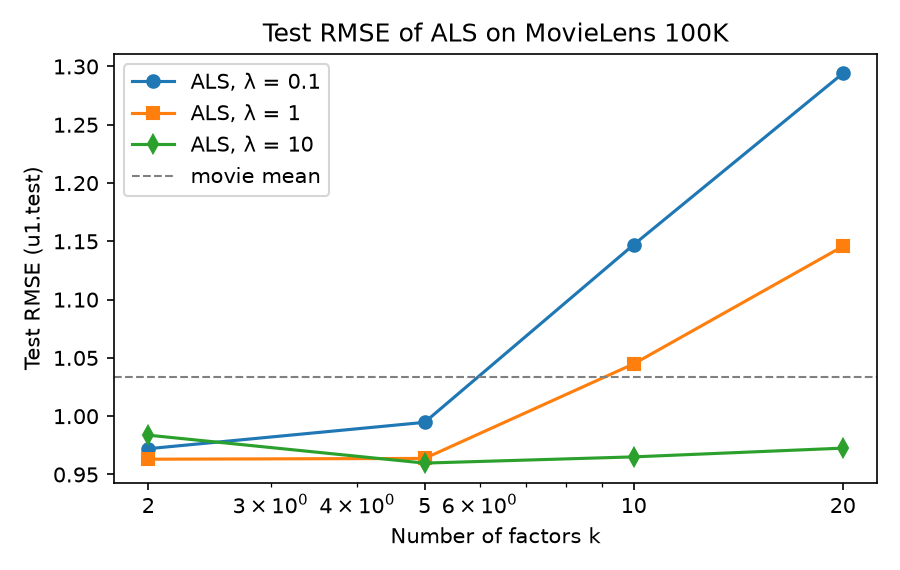
\includegraphics[width=0.6\textwidth]{figures/als_test_rmse_real.png}
  \caption{Test RMSE of ALS against $k$, one line per $\lambda$; the dashed line is the movie-mean
  baseline.}
  \label{fig:grid}
\end{figure}

Table~\ref{tab:grid} and Figure~\ref{fig:grid} show both sides of the role of $\lambda$.

\begin{itemize}[leftmargin=*]
  \item \textbf{Overfitting.} At $\lambda = 0.1$ the training RMSE falls from 0.874 to 0.466 as $k$
        grows from 2 to 20, while the test RMSE rises from 0.972 to 1.294, worse than the
        movie-mean baseline. A user with 4 ratings described by 20 factors has more unknowns than
        data, and with almost no penalty the factors bend to fit those ratings.
  \item \textbf{Regularization.} At $\lambda = 10$ the test RMSE stays between 0.960 and 0.984 for
        every $k$, and the training RMSE stays higher (0.717 at $k = 20$): the penalty does not let
        the model memorize.
  \item \textbf{Underfitting.} At $k = 2$, $\lambda = 10$ is worse than $\lambda = 1$ (0.984 against
        0.963). With only two factors there is little to overfit, and a strong penalty removes
        useful signal.
  \item \textbf{The best $k$ depends on $\lambda$:} $k = 2$ at $\lambda = 0.1$ and $\lambda = 1$,
        $k = 5$ at $\lambda = 10$. A stronger penalty lets the model afford more factors.
\end{itemize}

The lowest test RMSE is \textbf{0.9598}, at $k = 5$ and $\lambda = 10$, 7.1\% below the movie-mean
baseline. Three cautions apply. First, several settings are within 0.005 of it ($k = 2$,
$\lambda = 1$: 0.9631; $k = 5$, $\lambda = 1$: 0.9638), and only the confidence intervals of
Proposition~8 can say whether gaps that small are real. Second, choosing $k$ and $\lambda$ by the
test RMSE lets the test set influence the choice; tuning them properly would need a validation
split of \code{u1.base}. Third, for $k \ge 5$ the best $\lambda$ is the largest one tried, so a
larger $\lambda$ might do better still.

\placeholder{Emmanuel}{The 95\% confidence interval of Proposition~8 for the test RMSE of each
method, at least for the best ALS model and the baselines.}

\placeholder{Jagadeesh}{The mean-filled truncated SVD (Method~3, from scratch) on the same split,
for the same values of $k$, with its test RMSE next to ALS.}

\subsection{The objective never increases}

Across all 12 runs, $J$ did not increase at any of the 1{,}044 half-steps (Theorem~4).
Figure~\ref{fig:real-objective} shows the run with the lowest test RMSE.

\begin{figure}[htbp]
  \centering
  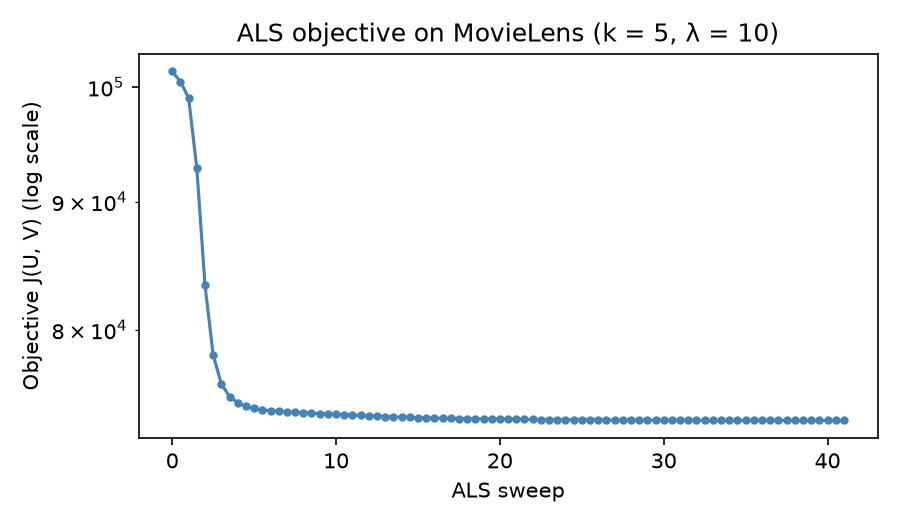
\includegraphics[width=0.62\textwidth]{figures/als_objective_real.png}
  \caption{The ALS objective on MovieLens after every half-step, $k = 5$, $\lambda = 10$.}
  \label{fig:real-objective}
\end{figure}

\subsection{Comparison with the library}

For every one of the 943 user systems and 1{,}682 movie systems of the best model we solved
$Gx = h$ with \code{my\_gauss\_solve} and with \code{numpy.linalg.solve}. For user~1 the largest
difference was $2.2\times 10^{-16}$; over all 2{,}625 systems it was $8.9\times 10^{-16}$, below the
pass threshold of $10^{-10}$. The largest condition number of any $G$ was 6.3, so by
Remark~\ref{rem:rounding} differences up to about $6.3 \times 2.2\times10^{-16} \approx 1.4\times
10^{-15}$ are expected; the observed difference is smaller. The condition numbers are small because
of Proposition~2: every eigenvalue of $G$ is at least $\lambda = 10$. The regularization that
prevents overfitting also keeps every system easy to solve accurately.

\owner{Muhammad Saad Malik}{\tbd{checker}}

% ============================================================================
\section{Assumption Checks}
\label{sec:assumptions}

Section~3 of Iteration~2 listed seven assumptions and how each would be checked. Here we run the
checks for the four that concern ALS. They are implemented once, in \code{src/assumptions.py}, and
run first on the simulation, where every assumption holds by construction, so that we know what
passing looks like, and then on MovieLens. Table~\ref{tab:assumptions} summarizes the results.

\begin{table}[htbp]
\centering
\small
\begin{tabular}{@{}>{\raggedright}p{2.3cm}>{\raggedright}p{3.3cm}>{\raggedright}p{3.4cm}>{\raggedright}p{3.8cm}>{\raggedright\arraybackslash}p{1.8cm}@{}}
\toprule
Assumption & Check & Simulation & MovieLens & Verdict \\
\midrule
1.\ Low rank & Held-out RMSE against $k$ has an interior minimum
  & Lowest at $k = 3$, the true rank & Lowest at $k = 5$ for $\lambda = 10$; at $k = 2$ (the edge)
  for $\lambda = 0.1$ and $1$ & Supported \\
\addlinespace
3.\ Bilinear interaction & Residual $r - \hat r$ against $\hat r$: bin means and calibration slope
  & Slope 1.068 (1.000 for the truth itself) & Slope 1.182; bin means from $-0.27$ to $+0.14$
  & Mostly holds \\
\addlinespace
4.\ $\lambda > 0$ & Rows with fewer than $k$ ratings; smallest eigenvalue of any $G$
  & 0 rows; smallest eigenvalue 4.99 $\ge \lambda = 1$ & 1 user and 399 movies below $k = 5$;
  smallest eigenvalue $10.0000 = \lambda$ & Needed, and satisfied \\
\addlinespace
5.\ Equal-weight squared error & Share of $\sum e^2$ carried by the largest 5\% of errors
  & 43.4\% (27.3\% for the truth itself) & 30.0\%; skewness $-0.49$ & Holds \\
\bottomrule
\end{tabular}
\caption{Assumption checks for ALS. For normal errors the share in the last row is 27.9\%.}
\label{tab:assumptions}
\end{table}

\subsection{What passing looks like}
\label{sec:passing}

The residuals of a fitted model mix two things: the noise in the data, and the estimator's own
error. On the simulation we can separate them, because we can also predict with $R_{\mathrm{true}}$
itself, whose residuals are the noise alone. We summarize the residuals with two numbers.

\begin{itemize}[leftmargin=*]
  \item The \emph{calibration slope} $b = \sum(\hat r - \bar{\hat r})(r - \bar r) \big/
        \sum (\hat r - \bar{\hat r})^2$ is the least-squares slope of $r$ against $\hat r$.
        The residual $r - \hat r$ then has slope $b - 1$ against $\hat r$, so $b = 1$ means no
        linear trend. $b > 1$ means the predictions are too timid, pulled too far towards $\mu$;
        $b < 1$ means they are too extreme.
  \item The \emph{share of the largest 5\%} is the fraction of $\sum e^2$ carried by the 5\% of
        errors with the largest $|e|$. For $Z \sim \mathcal N(0, \sigma^2)$ it is the same for
        every $\sigma$: with $z = \Phi^{-1}(0.975) \approx 1.96$, integration by parts gives
        $\int_z^\infty t^2 \varphi(t)\,dt = z\varphi(z) + 1 - \Phi(z)$, so the share is
        $2\bigl[z\varphi(z) + 1 - \Phi(z)\bigr] \approx 0.279$. A much larger share means that a
        few large errors dominate the RMSE.
\end{itemize}

\begin{table}[htbp]
\centering
\begin{tabular}{@{}lcccc@{}}
\toprule
Predictor & Slope & Largest $|$bin mean$|$ & Excess kurtosis & Largest 5\% \\
\midrule
$R_{\mathrm{true}}$ itself (residual = noise) & 1.000 & 0.011 & $-0.09$ & 27.3\% \\
ALS, $k = 3$, $\lambda = 1$ & 1.068 & 0.230 & $+5.46$ & 43.4\% \\
ALS, $k = 3$, $\lambda = 0.01$ & 1.004 & 0.037 & $+0.24$ & 29.2\% \\
\bottomrule
\end{tabular}
\caption{Residuals on the hidden entries of the simulation: the data against the estimator.}
\label{tab:passing}
\end{table}

Table~\ref{tab:passing} shows that the data pass both checks exactly. The fitted model with
$\lambda = 1$ does not: its slope is 1.068 and its largest 5\% of errors carry 43.4\%. With
$\lambda = 0.01$ both deviations almost vanish, so they come from the regularization, not from the
data. Shrinkage towards $\mu$ costs the most where the true value is far from $\mu$ and where a
row has few ratings, which tilts the residuals and fattens their tails. The lesson for the real data
is that a residual check tests the data and the estimator together: for a regularized model,
passing looks like a slope somewhat above 1, not exactly 1.

\subsection{Assumption 1: low-rank structure}

On the simulation the held-out RMSE for $k = 1, \dots, 6$ is 1.633, 1.131, 0.181, 0.193, 0.197,
0.202: an interior minimum exactly at the true rank, $k = 3$. On MovieLens, at $\lambda = 10$, the
test RMSE is 0.984, 0.960, 0.965, 0.973 for $k = 2, 5, 10, 20$: an interior minimum at $k = 5$. At
$\lambda = 0.1$ and $\lambda = 1$ the lowest value is at $k = 2$, the edge of the grid. That is not
evidence against low rank: with a weak penalty the data support very few factors before
overfitting starts. A handful of factors, between 2 and 5, captures what the ratings can teach,
and nothing suggests that more would help.

\subsection{Assumption 3: bilinear interaction}

On MovieLens the calibration slope of the test residuals is 1.182, and the mean residual in the ten
bins of $\hat r$ runs from $-0.207$, $-0.270$, $-0.215$ for the lowest predictions to $+0.085$,
$+0.122$, $+0.096$, $+0.140$ for the upper-middle ones: low predictions should be lower and high
ones higher. This is the shrinkage pattern of Section~\ref{sec:passing}, and $\lambda = 10$ is a
much stronger penalty than the simulation's $\lambda = 1$, so a larger slope is expected. Relative
to the noise the trend is small: the largest bin mean is 0.27 against a residual standard deviation
of 0.96. The top bin flattens to $+0.023$ because ratings stop at 5. The residual plot
(Figure~\ref{fig:assumptions-real}, middle) shows five diagonal stripes; they are not a pattern in
the errors but a consequence of whole-star ratings, since for every rating $r \in \{1,\dots,5\}$ the
residual $r - \hat r$ lies on a line of slope $-1$. On real data there is no true matrix to predict
with, so the shrinkage explanation is supported by the direction of the trend rather than proven.
Our verdict: no strong evidence against bilinear structure, and a mild trend that matches the
regularization.

\subsection{\texorpdfstring{Assumption 4: $\lambda > 0$}{Assumption 4: lambda > 0}}
\label{sec:a4}

On the simulation no user or movie has fewer than $k = 3$ ratings, and the smallest eigenvalue of
any $G$ is 4.99, above $\lambda = 1$. On MovieLens at $k = 5$, one user and 399 movies have fewer
than 5 training ratings, and at $k = 20$, 109 users and 814 movies have fewer than 20. For all of
these rows $V_u\T V_u$ (or $U_i\T U_i$) has rank below $k$ and is singular, so without $\lambda$ the
updates would have no unique answer. The smallest eigenvalue of any $G$ is exactly $10.0000$. It
belongs to the 32 movies with no training ratings, for which $G = \lambda I_k$, so the bound of
Proposition~2 is not only satisfied but attained.

\subsection{Assumption 5: equal-weight squared error}

On MovieLens the test residuals have mean $-0.036$, standard deviation 0.959, skewness $-0.49$ and
excess kurtosis $+0.10$, and their largest 5\% carry 30.0\% of $\sum e^2$, close to the 27.9\% of
normal errors. A handful of large misses therefore does not dominate the RMSE, which is the failure
Iteration~2 warned about. The departure from a bell shape that Iteration~2 expected appears as
skewness rather than heavy tails. Ratings are bounded and $\mu \approx 3.53$, so the worst miss
downwards (an unexpected 1 star, about $-2.5$) is larger than the worst miss upwards (about $+1.5$),
and the left tail is longer. The real residuals have lighter tails than the regularized simulation
(30.0\% against 43.4\%) because on a 1--5 scale no error can exceed 4, while the simulated values
are unbounded.

\begin{figure}[htbp]
  \centering
  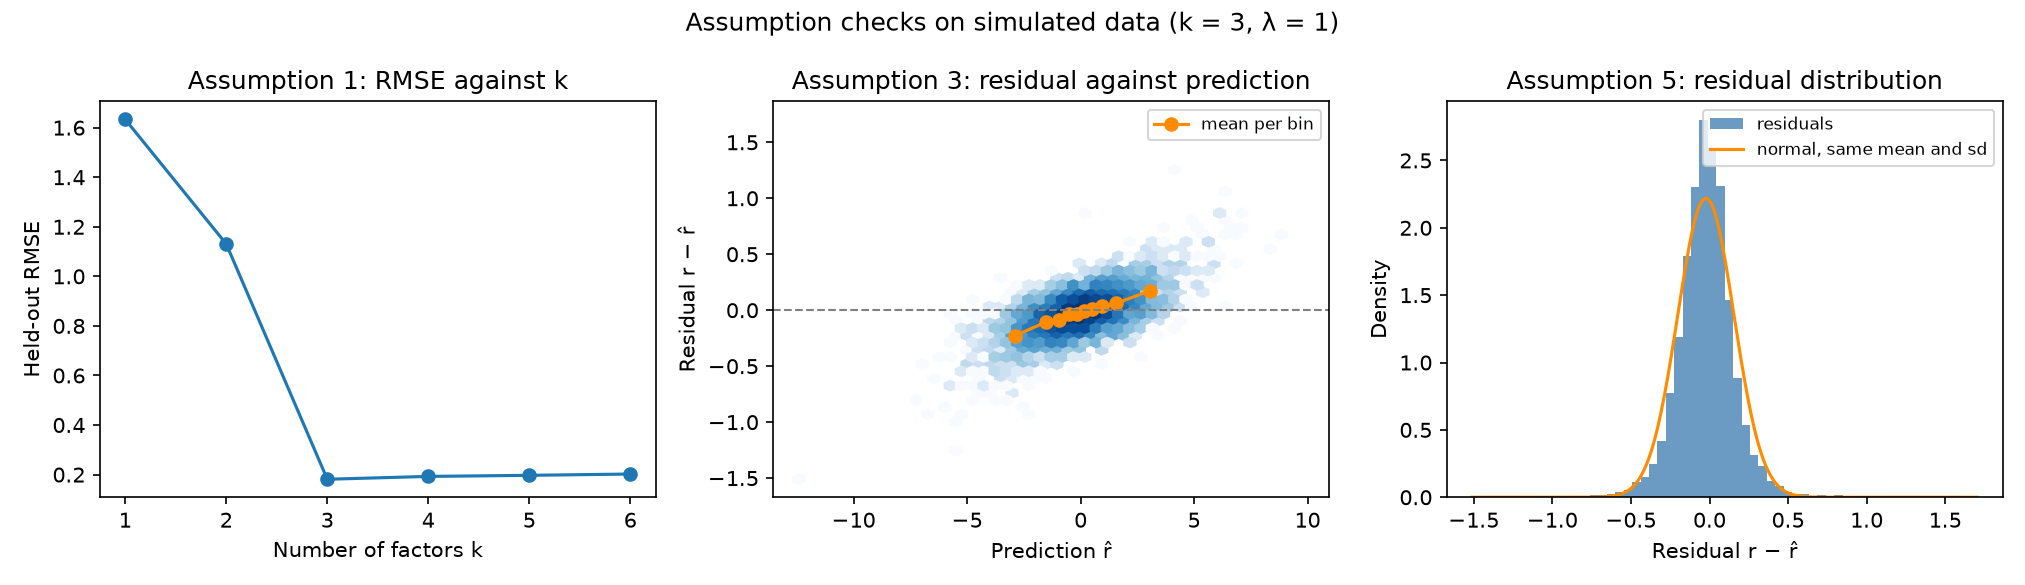
\includegraphics[width=\textwidth]{figures/assumptions_simulation.png}
  \caption{Assumption checks on the simulation ($k = 3$, $\lambda = 1$, residuals on the hidden
  entries).}
  \label{fig:assumptions-sim}
\end{figure}

\begin{figure}[htbp]
  \centering
  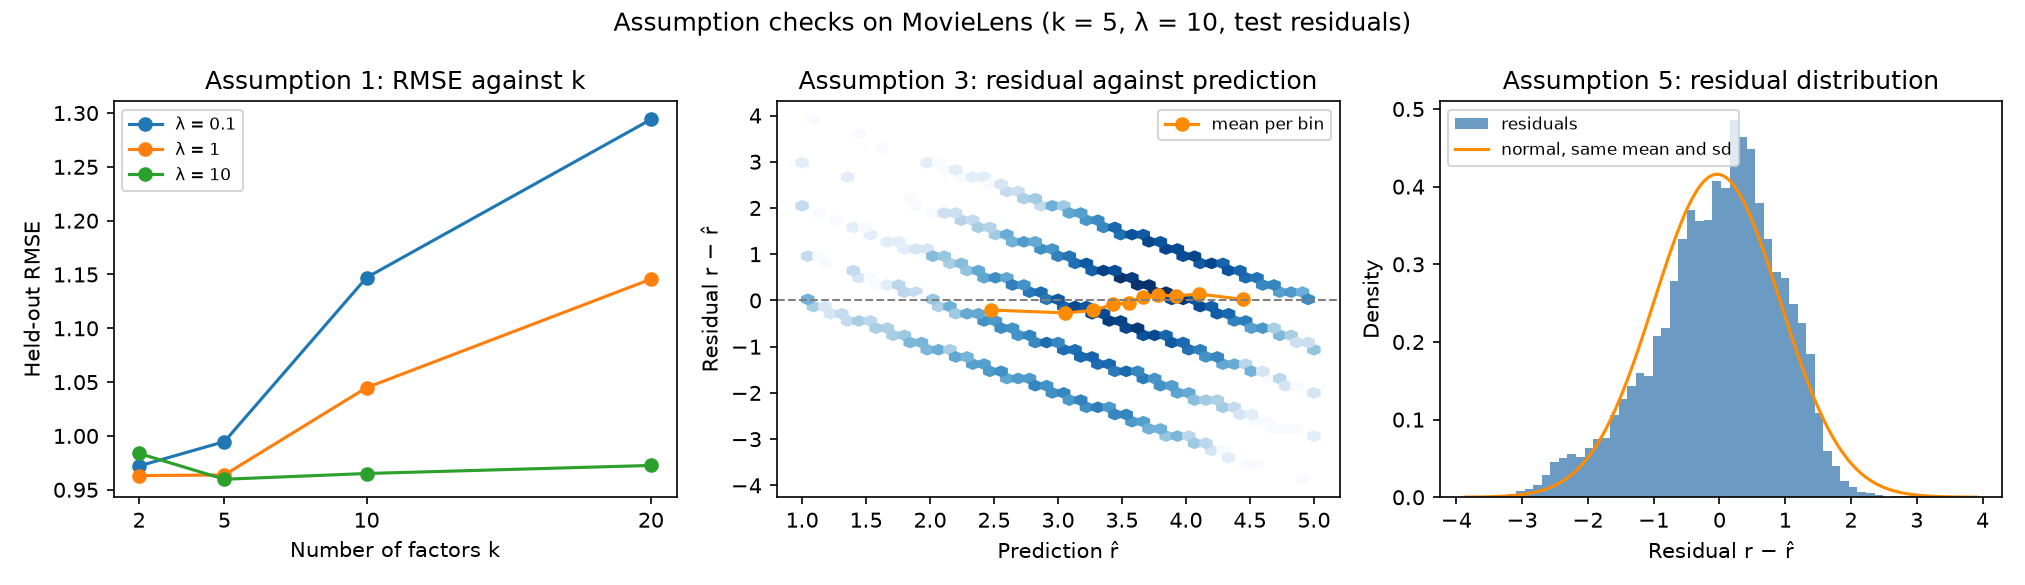
\includegraphics[width=\textwidth]{figures/assumptions_real.png}
  \caption{Assumption checks on MovieLens ($k = 5$, $\lambda = 10$, test residuals).}
  \label{fig:assumptions-real}
\end{figure}

\owner{Muhammad Saad Malik}{\tbd{checker}}

\placeholder{Emmanuel and Jagadeesh}{Assumption~2 (missing at random: rating distributions of
popular and rarely rated movies), Assumption~6 (the confidence interval against the spread of the
RMSE over repeated splits) and Assumption~7 (the ratios $\sigma_{j+1}/\sigma_j$ and the iterations
each factor needs), on the simulation first and then on MovieLens.}

% ============================================================================
\section{Iteration 3 -- Math Questions}
\label{sec:questions}

These are the five questions listed for Project~12 in the Iteration~3 handout.

\paragraph{Q1. For a $3\times3$ rating matrix with 2 missing entries and $k = 1$, run one full ALS
step and print $U$, $V$ and the objective.}

Section~\ref{sec:example} works it in full, and \code{src/small\_example.py} prints every step. One
full step (Steps 3 and 4) from $v^{(0)} = (1,1,1)\T$ with $\lambda = 1$ gives
\[
U^{(1)} = (3,\ 2,\ 1)\T, \qquad V^{(1)} = \bigl(\tfrac85,\ \tfrac{14}{11},\ \tfrac56\bigr)\T,
\qquad J: \ 27 \ \to\ \tfrac{6803}{330} \approx 20.62,
\]
and both second-way checks pass exactly: every row satisfies its normal equations, and $J$
decreased.

\owner{Muhammad Saad Malik}{\tbd{checker}}

\paragraph{Q2. Implement ALS from scratch (your own Gaussian elimination for each small system).
Compare one update with \code{numpy.linalg.solve}.}

The implementation is described in Section~\ref{sec:impl}; every small system is solved by
\code{my\_gauss\_solve} (Section~\ref{sec:gauss}), never by \code{numpy.linalg}, and
Proposition~\ref{prop:pivot} shows that it cannot fail for $\lambda > 0$. The comparison with
\code{numpy.linalg.solve}:

\begin{center}
\begin{tabular}{@{}lcc@{}}
\toprule
Data & One update (user 1) & All row updates \\
\midrule
Simulation ($k = 3$, $\lambda = 1$, 180 systems) & 0 (identical) & $8.9\times10^{-16}$ \\
MovieLens ($k = 5$, $\lambda = 10$, 2{,}625 systems) & $2.2\times10^{-16}$ & $8.9\times10^{-16}$ \\
\bottomrule
\end{tabular}
\end{center}

All differences are far below $10^{-10}$. They are not exactly zero because floating-point
arithmetic rounds every operation, and \code{numpy.linalg.solve} calls a LAPACK routine that
performs the same elimination in a different order. By Remark~\ref{rem:rounding} the two can
differ by about $\operatorname{cond}(G)\,\varepsilon$; with $\operatorname{cond}(G) \le 6.3$ that
is about $1.4\times 10^{-15}$. The exact digits also vary between machines, because each platform
ships its own LAPACK, but they stay at this level.

\owner{Muhammad Saad Malik}{\tbd{checker}}

\paragraph{Q3. Build a truncated-SVD baseline by filling missing ratings with the mean.}
This question belongs to the truncated-SVD part of the project (Method~3).

\placeholder{Jagadeesh}{The answer to Q3: Method~3 from scratch on the simulation and on
MovieLens. A reference value already exists: with \code{numpy.linalg.svd}, the mean-filled rank-3
SVD has RMSE 1.394 on the hidden entries of the simulation, against 0.150 for ALS.}

\paragraph{Q4. Split ratings into train and test sets and compute the test RMSE.}

We use the provided split: \code{u1.base} for training (80{,}000 ratings) and \code{u1.test} for
testing (20{,}000), with no rating in both. The test RMSE is
$\bigl(\frac1N \sum_{(u,i)\in\Omega_{\mathrm{te}}} (r_{ui} - \hat r_{ui})^2\bigr)^{1/2}$ with
$N = 20{,}000$. The global mean gives 1.1537, the movie mean 1.0334, and ALS between 0.9598
($k = 5$, $\lambda = 10$) and 1.2940 ($k = 20$, $\lambda = 0.1$); Table~\ref{tab:grid} lists all
twelve settings and Section~\ref{sec:real} discusses them.

\owner{Muhammad Saad Malik}{\tbd{checker}}

\paragraph{Q5. Plot the objective after each ALS iteration and confirm that it never increases.}

Figure~\ref{fig:sim-objective} (simulation) and Figure~\ref{fig:real-objective} (MovieLens) plot
$J$ after every half-step. $J$ did not increase at any of the 100 half-steps of the simulation or
the 1{,}044 half-steps of the twelve MovieLens runs. The check is also built into the code:
\code{my\_als} stops with an error if $J$ ever rises by more than $10^{-9}J$, which would mean a
bug, since Theorem~4 rules it out. It never stopped.

\owner{Muhammad Saad Malik}{\tbd{checker}}

% ============================================================================
\section{Verification Table}
\label{sec:verification}

\begin{table}[htbp]
\centering
\small
\begin{tabular}{@{}>{\raggedright}p{2.5cm}>{\raggedright}p{3.4cm}>{\raggedright}p{3.4cm}>{\raggedright}p{3.8cm}c@{}}
\toprule
Data & Quantity & Compared with & Difference & Pass? \\
\midrule
Small example & $Gx - h$, all 6 rows & 0, exact fractions & 0 & \checkmark \\
Small example & $J$ after Step 4 & $J$ after Step 3 & $6803/330 \le 27$ & \checkmark \\
\addlinespace
Simulation & $J$ after each half-step & Previous $J$ & 0 increases in 100 & \checkmark \\
Simulation & $\hat r$ on hidden entries & $R_{\mathrm{true}}$ & RMSE $= 0.150$ ($< 0.3$) & \checkmark \\
Simulation & Every row update & \code{numpy.linalg.solve} & $\max|\cdot| = 8.9\times10^{-16}$ & \checkmark \\
Simulation & Filled SVD on hidden entries & ALS on hidden entries & 1.394 against 0.150 & \checkmark \\
Simulation (4 sizes) & RMSE on hidden entries & $|\Omega|$ & log--log slope $-0.62$ & \checkmark \\
Simulation (stress test) & Fraction where ALS stops recovering & 531 unknowns & Between 20\% (1{,}530
  ratings) and 15\% (1{,}151) & \checkmark \\
Simulation & Smallest eigenvalue of $G$ & $\lambda = 1$ & $4.99 \ge 1$ & \checkmark \\
\addlinespace
Real data (12 runs) & $J$ after each half-step & Previous $J$ & 0 increases in 1{,}044 & \checkmark \\
Real data & Every row update & \code{numpy.linalg.solve} & $\max|\cdot| = 8.9\times10^{-16}$ & \checkmark \\
Real data & ALS test RMSE ($k = 5$, $\lambda = 10$) & Movie-mean baseline & 0.960 against 1.033 & \checkmark \\
Real data & Smallest eigenvalue of $G$ & $\lambda = 10$ & $10.0000 \ge 10$ & \checkmark \\
\addlinespace
\multicolumn{5}{@{}p{\dimexpr\linewidth\relax}@{}}{\tbd{Jagadeesh: rows for Method 3 ($\sigma_j$ and
singular vectors against \code{numpy.linalg.svd}).}} \\
\multicolumn{5}{@{}p{\dimexpr\linewidth\relax}@{}}{\tbd{Emmanuel: rows for Method 1 and the confidence
intervals.}} \\
\bottomrule
\end{tabular}
\caption{Every comparison in this report. Each number is printed by one of our scripts.}
\label{tab:verification}
\end{table}

% ============================================================================
\section*{AI Use Disclosure}

{\sloppy This topic was new to us, so we again used an AI assistant, Claude (Anthropic), throughout this
iteration. We used it to learn how ALS works step by step, including working through the small
example by hand, and to break the iteration into tasks. It helped us write the code in
\code{src/methods.py}, \code{src/simulate.py}, \code{src/small\_example.py},
\code{src/check\_simulation.py}, \code{src/run\_real.py} and \code{src/assumptions.py}, which we ran
on our own machines and checked ourselves; every number in this report comes from those runs. It
drafted the \LaTeX{} for this report from our code's output and helped us update the README. We
reviewed all of this work, and each of us can explain any part of this report.
\tbd{Jagadeesh and Emmanuel: add a sentence for your own AI use, if any.}\par}

\end{document}
